\chapter{Curved mesh generation}
\section{Introduction}

The problem of curved mesh generation involves at least one issue - the placement of the boundary ``high-order" nodes. A description of a high-order boundary is required, and the optimal placement of high-order boundary nodes must be decided.

Additionally, we usually need to deal with one more issue - maintaining the quality of elements near the boundary after placing the high-order boundary nodes. The deformation of the initially polygonal/polyhedral boundary to get a curved boundary usually causes the quality of boundary elements to get reduced. In cases with a viscous boundary layer mesh, these elements even become invalid \cite{curve:persson, gmsh:untangling}. Thus, the deformation of the boundary must be propagated into the domain, to displace interior nodes upto at least some distance from the boundary.

In our knowledge, there are three types of methods to achieve regularization of the interior mesh. The first type uses models based on solid mechanics to try to achieve valid mesh movement, as explained in the previous chapter. The second type of technique to move the interior nodes involves interpolation of the boundary displacement to interior nodes, again, as previously explained. An interesting development in curved mesh generation by interpolation is due to Ims at. al. \cite{curve:meshcurve}, in which explicit interpolation (\cite{mm:explicit}) is used to curve the interior of the mesh. Finally, researchers have ``untangled" the near-boundary elements, and otherwise improved the quality of the mesh, by optimization processes. The cost function is usually some kind of curved-mesh quality measure. One prominent example of this is in the Gmsh meshing software \cite{gmsh:untangling}.

We present an alternative approach based on interpolation by radial basis functions. This approach is compared to the more prevalent methods of linear elasticity \cite{curve:hartmann}.

In the rest of the sections, we discuss the methodology used to generate 2D unstructured quadratic meshes from linear meshes, and then present examples to demonstrate the effectiveness of our method. We compare the quality of meshes given by the RBF interpolation method and the linear-elasticity method.

We initially preprocess the linear mesh to generate a straight-faceted high-order mesh. To do this, we introduce extra nodes along edges, in faces and inside cells as required. Next, we either use CAD data or use a high-order boundary reconstruction method to obtain the actual positions of boundary high-order nodes. Finally, interior nodes are moved according to the boundary displacement imposed because of the previous step.

\section{Spline reconstruction for boundaries of 2D meshes}
\label{subsec:spline2d}
Since only the linear mesh is taken as input, a high-order boundary representation first needs to be reconstructed from the piecewise linear $C^0$ boundary. For 2D meshes, we use a cubic spline reconstruction to get a smooth ($C^2$) parametric curve describing the boundary. All boundary nodes are used as spline control points, and we get a cubic function between every two consecutive boundary nodes. At the control points, we require the two spline curves meeting there to share a common tangent and curvature, thus enforcing $C^2$ continuity. Since it is common for the true boundary to be specified in terms of cubic spline curves, this is expected to give us an accurate reconstruction. Corners are detected by comparing the normal vectors of the two facets sharing a point. If the dot product between the two normal vectors is below a particular user-specified threshold, the point is considered as a corner and is not smoothed over by the reconstruction procedure. Alternatively, the user can list all the corner points as input. Thus the reconstructed boundary is piecewise $C^2$, which is found to work well for the test cases we considered. The spline reconstruction requires the solution of a symmetric positive definite linear system, of size equal to the number of boundary nodes in the curved part of the boundary, in order to calculate the cubic spline coefficients. The system(s) can be solved quickly using a conjugate gradient (CG) solver. More details are given in appendix \ref{app:spline}.

Instead of a global reconstruction by cubic splines, a local reconstruction at each boundary node could also be used. This is described briefly for 3D meshes in the last chapter, conclusions and future work.

Once we have the smooth reconstructed boundary, we calculate the final positions of the boundary nodes in the curved mesh. This is currently done by simply moving the high-order boundary nodes, originally at regular intervals on the boundary facet, to corresponding intervals in parameter space on the cubic spline curve associated with that facet. This method is found to be quite robust for the meshes tested. Thus, the boundary displacements are obtained. Alternatively, if the CAD geometry is available, the displacements can be computed using it.

\section{Interior mesh movement}

To propagate the boundary motion to the interior of the mesh, we favor interpolation by radial basis functions (RBFs) \cite{mm:rbf}. We have also used linear elasticity to propagate the mesh movement to the interior. The isotropic linear elasticity variational formulation, as given by Gockenbach \cite{gockenbach}, is implemented in a P2 Galerkin FEM code for generation of quadratic meshes. In this case however, the size of the linear system to be solved is proportional to the total number of nodes in the mesh.

Though the RBF method requires the solution of a linear system of size proportional to only the number of boundary points, extra computation is required to evaluate equation \eqref{eqn:rbf} at each of the interior nodes to compute their displacements. In comparison, elasticity-based methods directly give us the displacements. 

While solving certain problems with the RBF method, we find that the linear system to be solved is sometimes quite ill-conditioned, depending upon the mesh. Iterative Krylov-subspace solvers such as conjugate gradient (CG) and BiCGSTAB are not able to solve the system in such cases. However, in the cases that we worked on (such as curved mesh generation of hybrid meshes for viscous simulations of airfoils), sparse direct methods are capable of solving the system efficiently and effectively. This is likely to hold true in general as the systems to be solved will usually not be very large (having size of the number of boundary nodes).

The inability of iterative solvers to compute a solution can perhaps be explained by the discussion on condition numbers of RBF matrices in Wendland's paper \cite{rbf:errorwendland}. If
\begin{equation}
q := \min_{i\neq j} \lVert \bld{x}_{bi} - \bld{x}_{bj} \rVert_2
\end{equation}
is the minimum distance between two boundary points, and $\bld{A}$ is the RBF interpolation matrix \eqref{eqn:rbf_system} then for Wendland's C2 function, we will have
\begin{equation}
\begin{aligned}
\text{cond}_2 (\bld{A}) &= \mathcal{O}(q^{-5}) \quad \text{in 2D, and} \\
\text{cond}_2 (\bld{A}) &= \mathcal{O}(q^{-6}) \quad \text{in 3D}
\end{aligned}
\end{equation}
as seen from section 4 of \cite{rbf:errorwendland}. In the case that the CG solver did not work, we had a 2D mesh with $q \approx 4 \times 10^{-7}$. This means that the condition number can be as high as $10^{30}$! Since we used only point-Jacobi preconditioning, we expect CG to not work in this case. If a more potent preconditioner (such as incomplete Cholesky decomposition or LU-SGS \cite{lusgs_precon}) is used, CG might be expected to work. But we found that direct solvers such as sparse LU decomposition work very well, and adopted this instead.

We have also tried using the stiffened linear elasticity method described in subsection \ref{subsec:stiffelast}. In this work, this is implemented by scaling each component of the element stiffness matrix of each element by the scaling term $\left(\frac{J_0}{J_\kappa}\right)^\chi$. This is valid as we only need to run the linear elasticity code on straight-sided meshes, and this means that the Jacobian $J_\kappa$ is constant over the element.

\subsection[Unsuitability of DG-based methods for curved mesh generation]{Unsuitability of Delaunay-graph-based methods for curved mesh generation}
\label{subsec:dgmunsuitable}
%********* TODO: DESCRIBE WHY DGM AND DG-RBF FAIL FOR CURVED MESH GENERATION. DESCRIBE THE 2-STEP RBF-DG METHOD, AND WHY THAT DOES NOT WORK EITHER *********

Several variants of the Delaunay graph mapping method were also attempted for generating curved meshes. While Delaunay graph mapping (DGM) is a very efficient scheme for accomplishing many types of mesh movement, it has a characteristic because of which it is unsuitable for certain meshes and motions, especially curved mesh generation. This is the fact that the movement of a node depends only on the motion of the Delaunay element containing it, not necessarily on the motion of the nearest boundary facets.

In case of curved mesh generation for highly anisotropic viscous meshes, it is possible for some Delaunay triangulation facets make angles with the boundary that are very different from 90 degrees (see figure \ref{fig:wmesh-dg}). Then we may have at least two issues.
\begin{itemize}
	\item[1.] Interior points close to a boundary facet can be influenced by another boundary facet far away having a very different curvature.
	\item[2.] It may be the case that an interior point is not at all influenced by the closest boundary facet.
\end{itemize}
These issues lead to low curved mesh quality in certain regions, and even invalid elements. We could try using DG-RBF (interpolation by radial basis functions in a Delaunay graph) to help alleviate issue (1), but issue (2) would still persist.

Figure \ref{fig:wmesh} shows a viscous mesh of a 3-element airfoil. Figures \ref{fig:wmesh-dg} and \ref{fig:wmesh-zoomed} show a portion of its slat. Figure \ref{fig:wmesh-dg} shows the Delaunay graph and figure \ref{fig:wmesh-zoomed} shows the deformed mesh. We can see that the DG lines make an angle very different from 90 degrees with the boundary. It is clear how points originally in a straight line deform in an oscillatory manner because successive points depend on different Delaunay elements, and different Delaunay elements have different movements depending on which boundary nodes they are made up of.

\begin{figure}
	\centering
	\includegraphics[scale=0.28]{3-airfoil}
	\caption{Mesh of a 3-element airfoil}
	\label{fig:wmesh}
\end{figure}
\begin{figure}
	\centering
	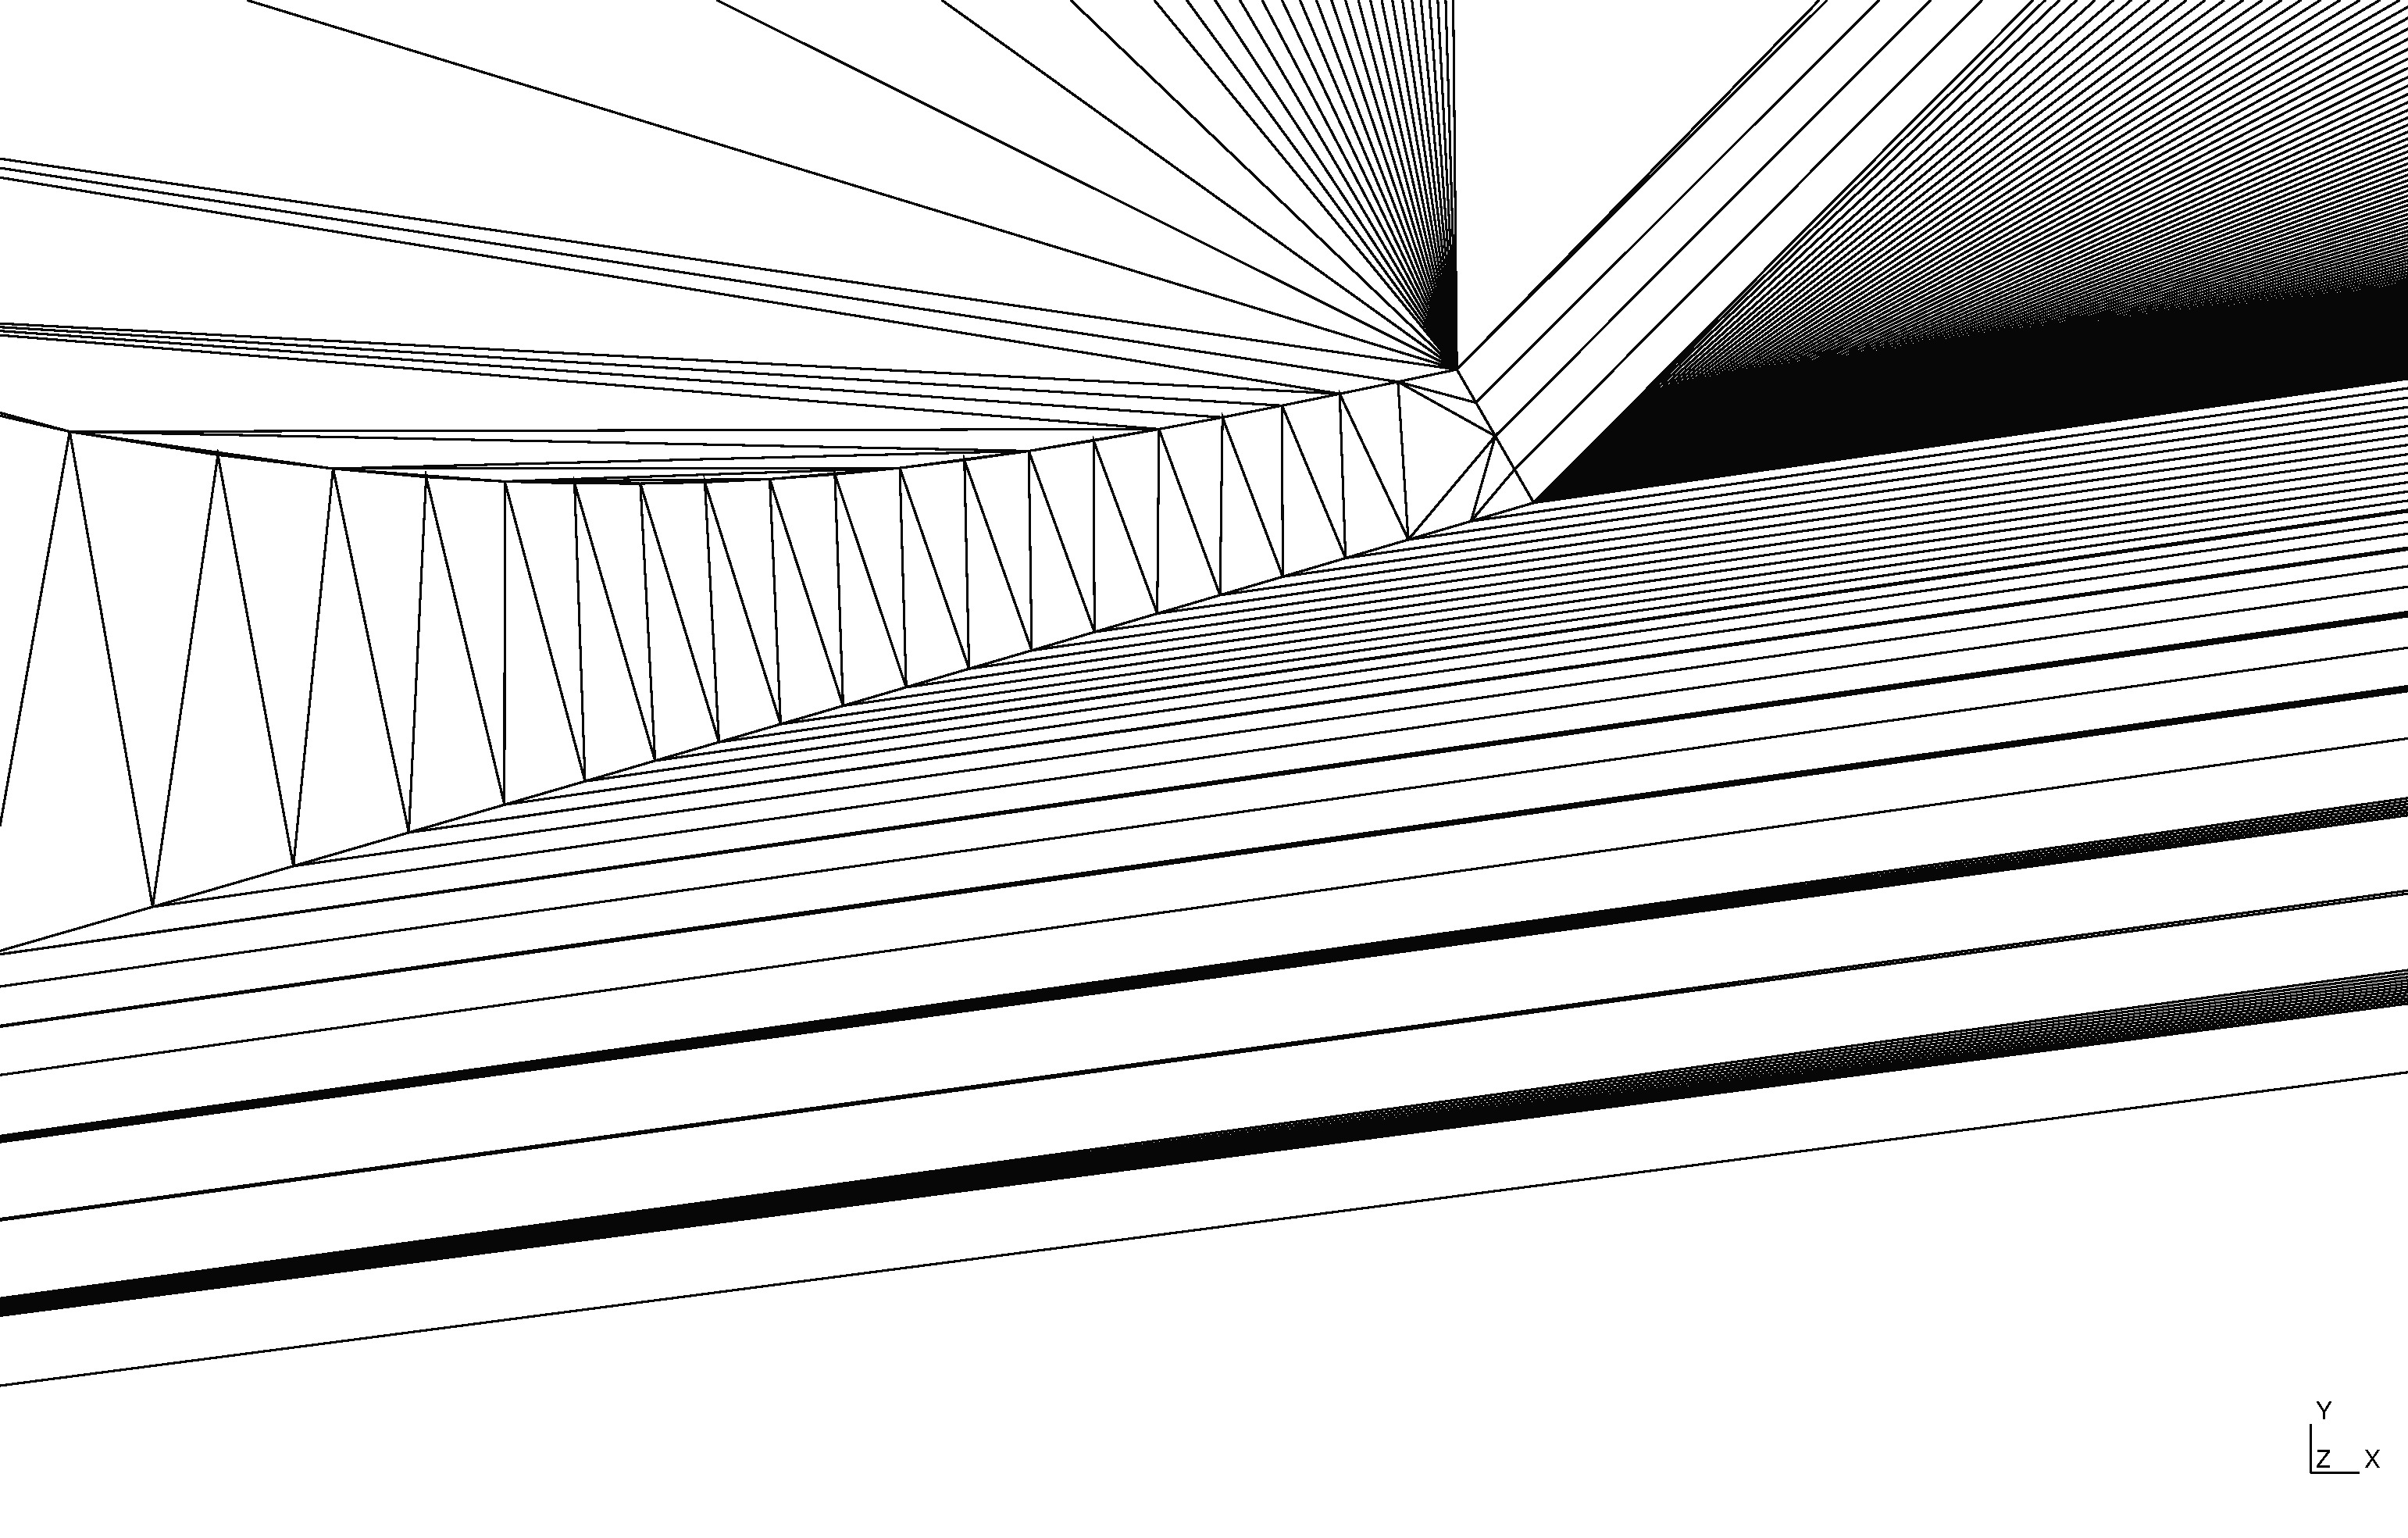
\includegraphics[scale=0.25]{dg-3airfoil-zoomed}
	\caption{Portion of the Delaunay graph near the lower part of the slat}
	\label{fig:wmesh-dg}
\end{figure}
\begin{figure}
	\centering
	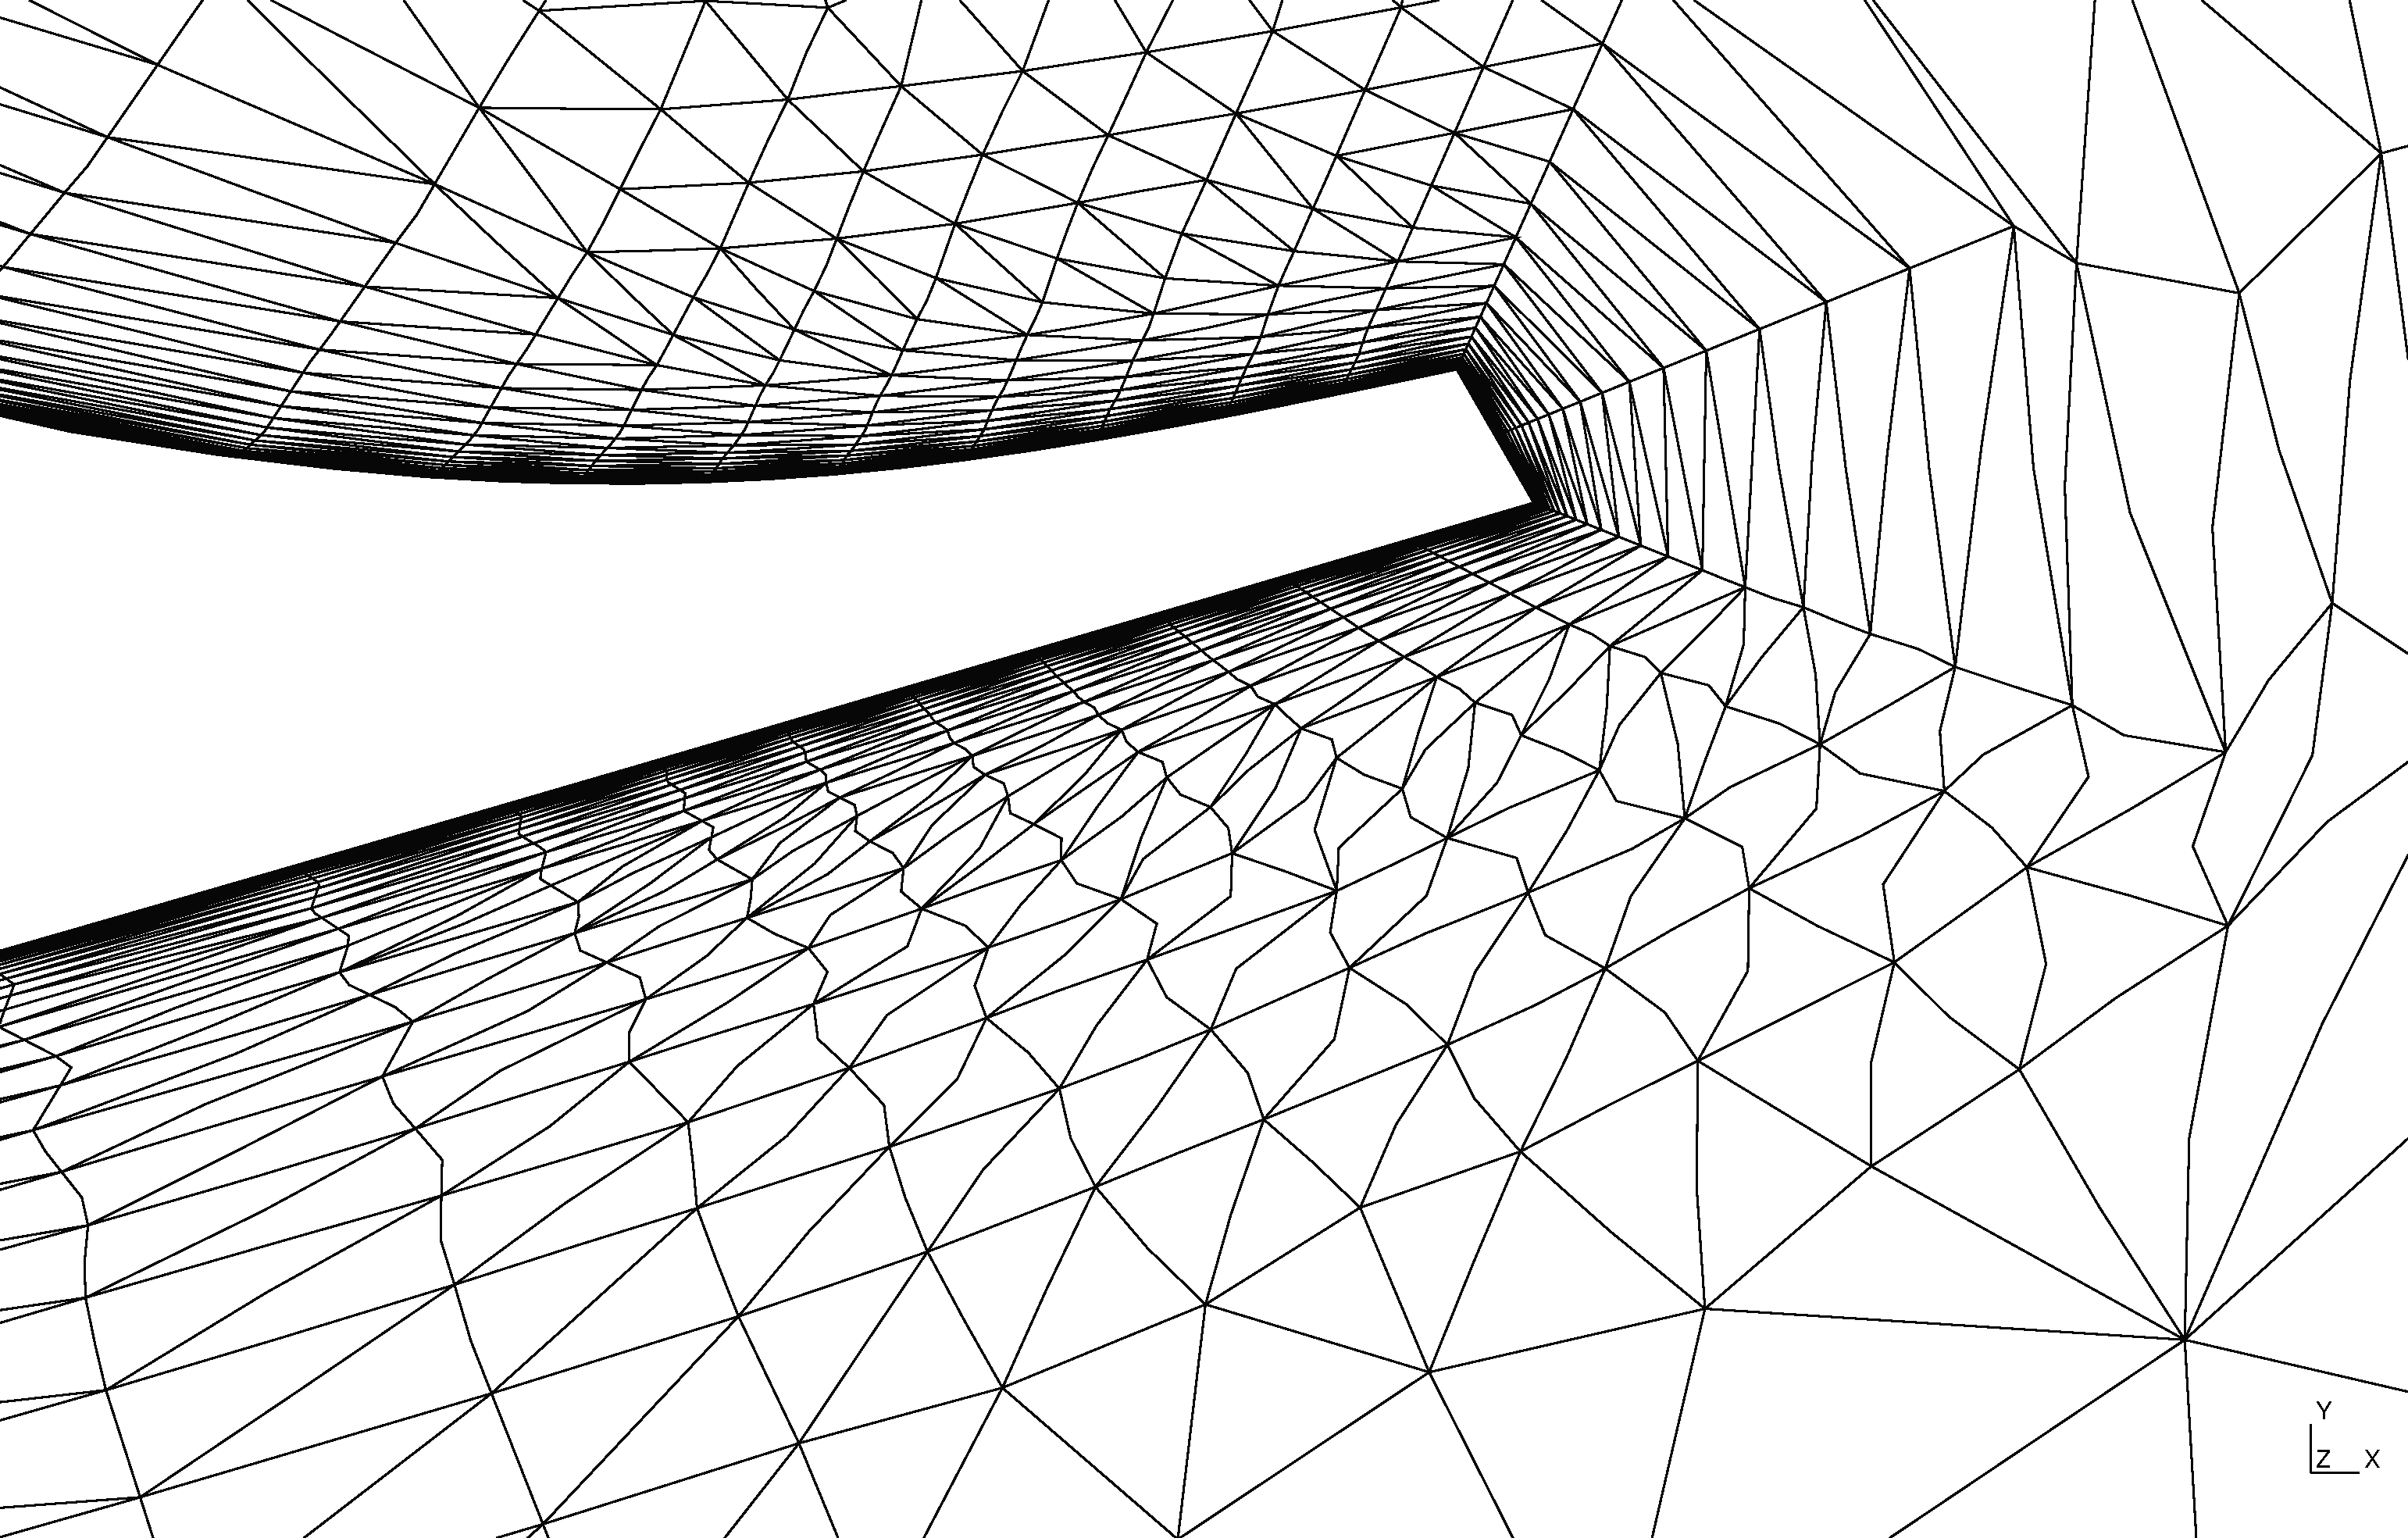
\includegraphics[scale=0.25]{mesh-3airfoil-zoomed}
	\caption{Portion of the generated mesh near the lower part of the slat}
	\label{fig:wmesh-zoomed}
\end{figure}

One way of improving this situation has been described in section \ref{sec:hybriddg}. However, the method of including a layer of interior points still does not work for curved mesh generation. This is simply to due to the high-frequency oscillatory nature of boundary displacements required for curved mesh generation and the fact that it is difficult to control how exactly the Delaunay graph (DG) elements are formed. It was found that some DG elements are formed by \emph{two high-order} boundary nodes and one interior node, as shown in \ref{fig:dg-curved-problem}. In the case shown, some interior nodes near the red circles (linear mesh nodes, called vertices) lie within a DG element that has nothing to do with the nearest boundary node, which is a boundary vertex in this case. A few interior nodes nearest to the boundary vertices are not inside the DG element, so they do not move because of the motion of the boundary. But beyond a small distance, the mesh nodes are in the DG element formed from two nearby high-order boundary nodes. This means that these nodes move with the DG element, and this creates a discontinuity in the interior node movement, leading to a bad boundary layer mesh.
\begin{figure}[!h]
	\centering
	\includegraphics[scale=0.3]{DG-curved-problem}
	\caption{Schematic diagram to show a possible Delaunay graph (dashed lines) and mesh (solid lines) near a boundary; circles represent regular boundary nodes; squares represent high-order boundary nodes}
	\label{fig:dg-curved-problem}
\end{figure}